\documentclass[10pt]{article}
\usepackage[a4paper,margin=0.9in]{geometry}
\usepackage[T1]{fontenc}
\usepackage{lmodern}
\usepackage{graphicx}
\usepackage{booktabs}
\usepackage[labelfont=bf,labelsep=period]{caption}
\renewcommand{\thefigure}{S\arabic{figure}}
\renewcommand{\thetable}{S\arabic{table}}
\newcommand{\bpb}{\textsc{bpb}}
\title{Supplement to ``Patch-Aware KV Cache Compression for Byte-Level Language Models''}
\author{Group 12, CS F429 Natural Language Processing, BITS Pilani Hyderabad Campus}
\date{}
\emergencystretch=3em
\begin{document}
\maketitle
Extra charts and the analytic compute table that did not fit in the main report.

\begin{figure}[h]
\centering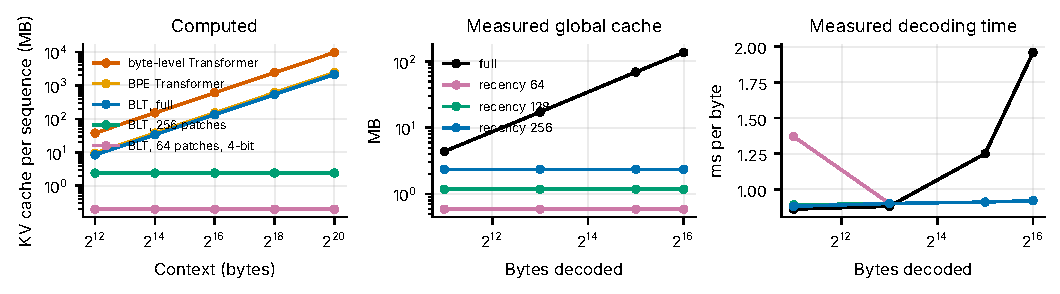
\includegraphics[width=\textwidth]{figures/fig_memory.pdf}
\caption{Cache memory. Left: computed KV size per sequence. Middle and right: measured on a GPU, one stream, real eviction of recency. A bounded cache holds the global cache at 0.59 to 2.36 MB while a full cache reaches 136.5 MB at 65,536 bytes; time per byte stays at 0.9 ms against a rise to 2.0 ms. The first recency point includes warm-up.}
\end{figure}

\begin{figure}[h]
\centering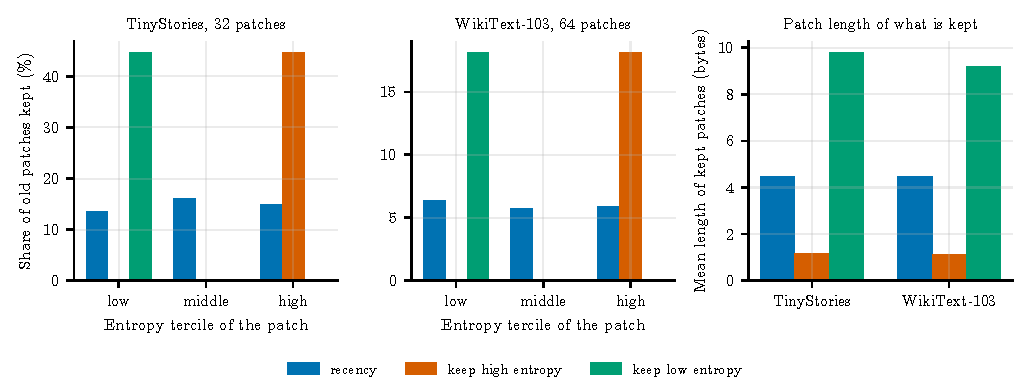
\includegraphics[width=\textwidth]{figures/fig_kept.pdf}
\caption{What each rule keeps at the close of a document. Left and middle: the share of old patches kept, by entropy tercile; keep-high-entropy keeps only high-entropy patches (and keep-low-entropy the contrary). Right: mean length of the kept patches; the entropy rule hoards one-byte fragments.}
\end{figure}

\begin{figure}[h]
\centering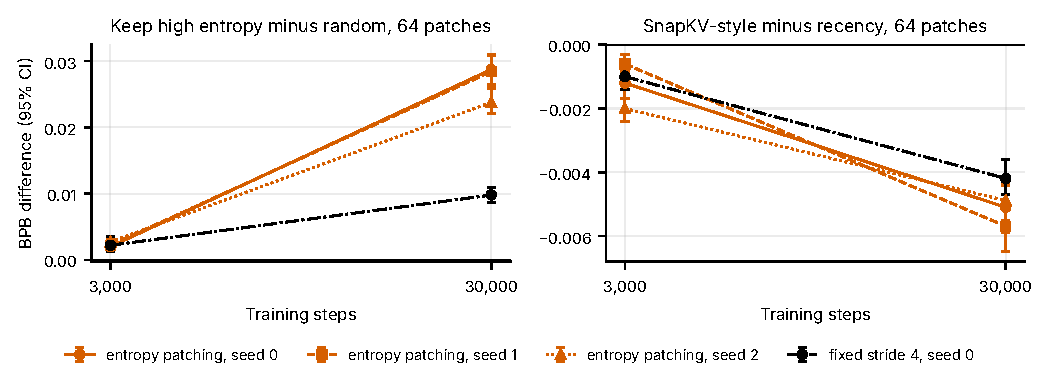
\includegraphics[width=\textwidth]{figures/fig_scale.pdf}
\caption{Ten times more training (3,000 to 30,000 steps, WikiText with code mix) makes the entropy penalty about ten times larger (left) and the SnapKV-style gain several times larger (right). Bars are 95\% bootstrap intervals; three seeds of entropy patching, one of fixed stride.}
\end{figure}

\begin{figure}[h]
\centering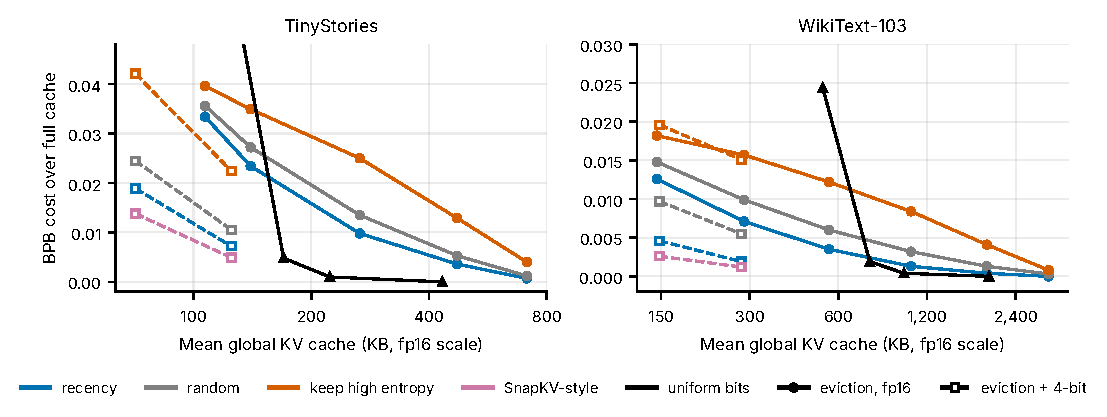
\includegraphics[width=\textwidth]{figures/fig_frontier.pdf}
\caption{Cost over the full cache against cache size (eviction and uniform rows are seed 0; 4-bit rows are the three-seed mean). Keeping high entropy (orange) is the worst eviction rule at every size and never on the frontier; SnapKV-style with 4-bit (pink, hollow) is the best low-memory point. Uniform 2 bits is off scale.}\label{fig:frontier}
\end{figure}

\begin{figure}[h]
\centering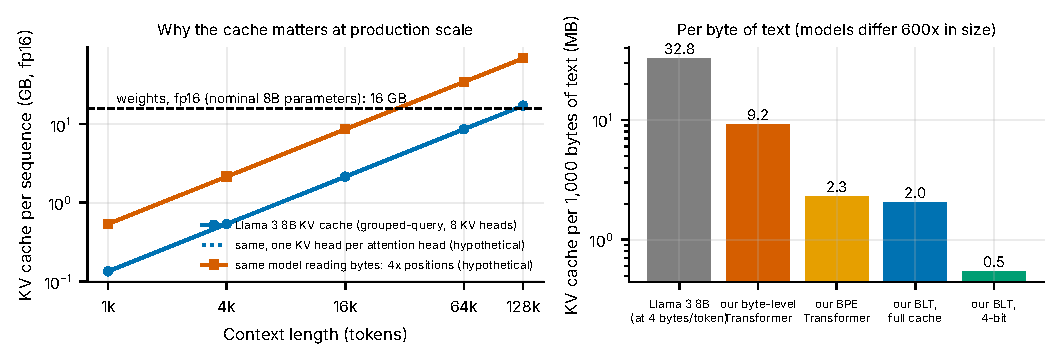
\includegraphics[width=\textwidth]{figures/fig_public.pdf}
\caption{Left: KV cache of a production-scale model grows linearly with context and passes the size of its weights near 128k tokens (computed from the Llama 3 8B configuration: 32 layers, 8 KV heads of dimension 128; fp16). A byte-reading version of the same model would need four times as many positions (hypothetical). Right: our small models per 1,000 bytes of text; the production figure assumes 4 bytes per token and is not comparable in quality, only in cost structure. The configuration is that of the published Llama 3 8B model.}\label{fig:public}
\end{figure}

\begin{figure}[h]
\centering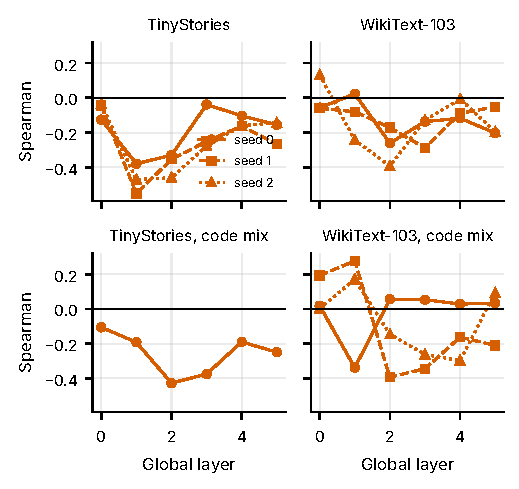
\includegraphics[width=0.62\textwidth]{figures/fig_attention.pdf}
\caption{Spearman correlation between the entropy of an old patch (at least 8 patches back) and the attention it receives, per global layer and seed. It is negative in the middle and upper layers of most models: the model reads predictable patches more than surprising ones. Correlational evidence only; the WikiText code-mix seed 0 model is the outlier.}
\end{figure}

\begin{figure}[h]
\centering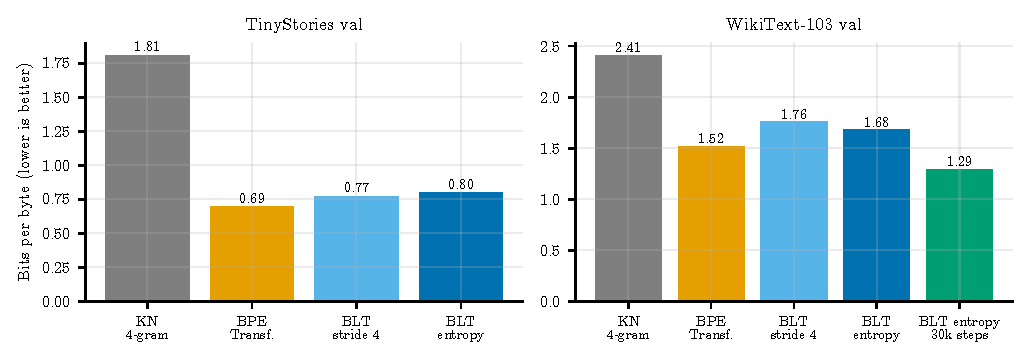
\includegraphics[width=\textwidth]{figures/fig_models.pdf}
\caption{Bits per byte of the classical baseline (Kneser-Ney byte 4-gram), the modern baseline (BPE Transformer) and the BLT-style models. At equal training (3,000 steps) the BPE Transformer is ahead; with ten times more training the WikiText code-mix BLT is lower (a comparison that gives the BLT more training and a code mix).}
\end{figure}

\begin{figure}[h]
\centering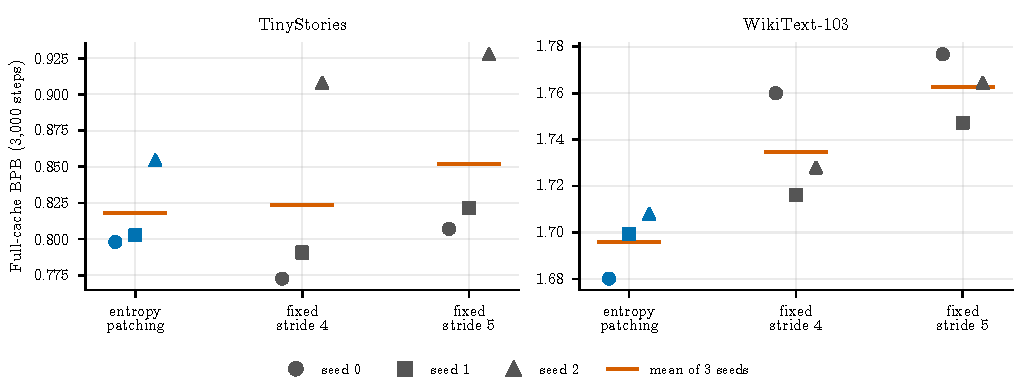
\includegraphics[width=\textwidth]{figures/fig_seeds.pdf}
\caption{Why we ran three seeds. Full-cache \bpb{} for every seed of each patching scheme: the seed spread (0.03 to 0.14) is as large as the gaps between schemes, so single-seed patching comparisons are not reliable. Entropy patching is lowest on WikiText in all three seed pairs.}
\end{figure}

\begin{figure}[h]
\centering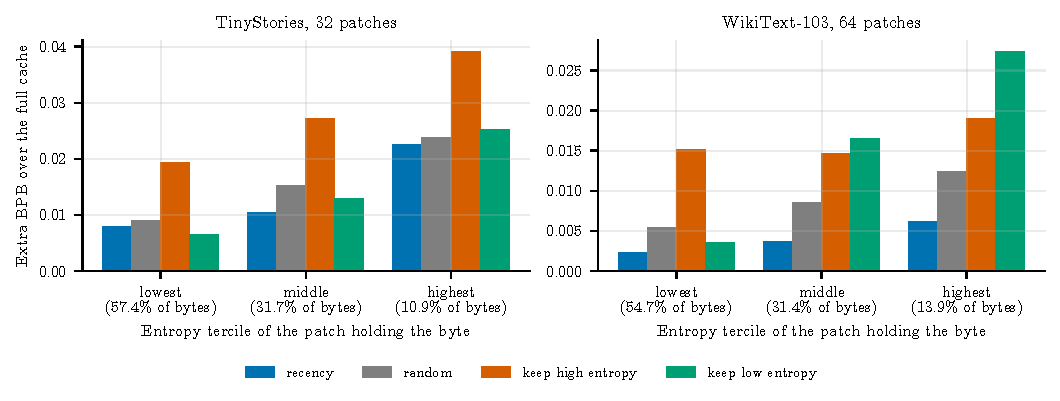
\includegraphics[width=\textwidth]{figures/fig_terciles.pdf}
\caption{Extra loss over the full cache, by the entropy tercile of the patch holding the byte (first patch and 8 newest protected). Keeping high-entropy patches does not protect the high-entropy bytes and also costs the easy bytes.}
\end{figure}

\begin{table}[h]
\centering\footnotesize
\caption{Analytic MFLOPs per generated byte and KV size (MB, fp16) at two contexts. The BPE Transformer was trained for 256 tokens (about 1,024 bytes), so its 4,096-byte rows are hypothetical.}
\resizebox{\textwidth}{!}{\begin{tabular}{@{}lrrrr@{}}
\toprule
 & \multicolumn{2}{c}{1,024 bytes} & \multicolumn{2}{c}{4,096 bytes}\\
Model & MFLOPs & MB & MFLOPs & MB\\
\midrule
BLT 13.3M, full global cache & 11.06 & 2.1 & 12.46 & 8.4\\
BLT, 64-patch cache & 10.73 & 0.6 & 10.73 & 0.6\\
BLT, full cache, plus entropy model & 19.58 & 2.1 & 20.98 & 8.4\\
BLT, 64-patch cache, plus entropy model & 19.25 & 0.6 & 19.25 & 0.6\\
BPE transformer 13.8M, full cache & 7.43 & 2.4 & 9.20 & 9.4\\
BPE transformer, 64-token cache & 6.99 & 0.6 & 6.99 & 0.6\\
Byte-level transformer, full cache & 30.87 & 9.4 & 59.18 & 37.7\\
Byte-level transformer, 64-entry cache & 22.02 & 0.6 & 22.02 & 0.6\\
Byte-level transformer, 288-entry cache (same text span as 64 patches) & 24.08 & 2.7 & 24.08 & 2.7\\
\bottomrule
\end{tabular}
}
\end{table}
\end{document}
